\documentclass[11pt,a4paper]{article}
			\usepackage[french]{babel}
					
				\usepackage{pifont}  
				\usepackage[utf8x]{inputenc}
				\usepackage[T1]{fontenc} 
				\usepackage{lmodern}			
				\usepackage{fancyhdr}
				\usepackage{textcomp}
				\usepackage{makeidx}
				\usepackage{tabularx}
				\usepackage{multicol}
				\usepackage{multirow}
				\usepackage{longtable}
				\usepackage{color}
				\usepackage{soul}
				\usepackage{boxedminipage}
				\usepackage{shadow}
				\usepackage{framed}			
				\usepackage{array}
				\usepackage{url}
				\usepackage{ragged2e}
				\usepackage{fancybox}
				\newcommand{\cadretitre}[2]{
				  \vspace*{0.8\baselineskip}
				  \begin{center}%
				  \boxput*(0,1){%
					%\colorbox{white}{\Large\textbf{\ #1\ }}%
				  }%
				  {%
					\setlength{\fboxsep}{10pt}%
				    \Ovalbox{\begin{minipage}{.8\linewidth}\begin{center}\Large\sffamily{#2}\end{center}\end{minipage}}}%
				  \end{center}
				  \vspace*{2\baselineskip}
				  }
			
			\makeatletter
			\def\@seccntformat#1{\protect\makebox[0pt][r]{\csname the#1\endcsname\quad}}
			\makeatother

				% Permet d'afficher qqchose à une positin absolue
				\usepackage[absolute]{textpos}
				\setlength{\TPHorizModule}{1cm}
				\setlength{\TPVertModule}{\TPHorizModule}
	
				\usepackage[titles]{tocloft}
				\setlength{\cftbeforesecskip}{0.5ex}
				\setlength{\cftbeforesubsecskip}{0.2ex}
				\addto\captionsfrench{\renewcommand\contentsname{}}
				
				\usepackage[font=scriptsize]{caption}
				
				\usepackage{listings}
\lstdefinestyle{lstverb}
  {
    basicstyle=\footnotesize,
    frameround=tttt, frame=trbl, framerule=0pt, rulecolor=\color{gray},
    lineskip=-1pt,   % pour rapprocher les lignes
    flexiblecolumns, escapechar=\\,
    tabsize=4, extendedchars=true
  }
\lstnewenvironment{Java}[1][]{\lstset{style=lstverb,language=java,#1}}{}
				\ifx\pdfoutput\undefined
					\usepackage{graphicx}
				\else
					\usepackage[pdftex]{graphicx}
				\fi
				\usepackage[a4paper, hyperfigures=true, colorlinks, linkcolor=black, citecolor=blue,urlcolor=blue, pagebackref=true, bookmarks=true, bookmarksopen=true,bookmarksnumbered=true,
                pdfauthor={}, pdftitle={TD Tableaux}, pdfkeywords={TD Tableaux, },pdfpagemode=UseOutlines,pdfpagetransition=Dissolve,nesting=true,
				backref, pdffitwindow=true, bookmarksnumbered=true]{hyperref}
				\usepackage{supertabular}
				\usepackage[table]{xcolor}
				\usepackage{url}
				\usepackage{caption} 
				\setlength{\parskip}{1.3ex plus 0.2ex minus 0.2ex}
				\setlength{\parindent}{0pt}
				
				\makeatletter
				\def\url@leostyle{ \@ifundefined{selectfont}{\def\UrlFont{\sf}}{\def\UrlFont{\footnotesize\ttfamily}}}
				\makeatother
				\urlstyle{leo}
				
				\definecolor{examplecolor}{rgb}{0.156,0.333,0.443}
				\definecolor{definitioncolor}{rgb}{0.709,0.784,0.454}
				\definecolor{exercisecolor}{rgb}{0.49,0.639,0}
				\definecolor{hintcolor}{rgb}{0.941,0.674,0.196}
				\definecolor{tableHeadercolor}{rgb}{0.709,0.784,0.454}
				\definecolor{tablerowAltcolor}{rgb}{.866,.905,.737}
				\definecolor{tablerowAlt2color}{rgb}{.968,.976,.933}
				\definecolor{verylightgray}{rgb}{0.98,0.98,0.98}
				
				\newenvironment{fshaded}{
				\def\FrameCommand{\fcolorbox{framecolor}{shadecolor}}
				\MakeFramed {\FrameRestore}}
				{\endMakeFramed}
				
				\newenvironment{fexample}[1][]{\definecolor{shadecolor}{rgb}{.913,.913,.913}
				\definecolor{framecolor}{rgb}{.156,.333,.443}
				\begin{fshaded}}{\end{fshaded}} 
				
				\newenvironment{fdefinition}{\definecolor{shadecolor}{rgb}{.913,.913,.913}
				\definecolor{framecolor}{rgb}{.709,.784,.454}
				\begin{fshaded}}{\end{fshaded}}
				
				\newenvironment{fexercise}{\definecolor{shadecolor}{rgb}{.913,.913,.913}
				\definecolor{framecolor}{rgb}{.49,.639,0}
				\begin{fshaded}}{\end{fshaded}}
				
				\newenvironment{fhint}{\definecolor{shadecolor}{rgb}{.913,.913,.913}
				\definecolor{framecolor}{rgb}{.941,.674,.196}
				\begin{fshaded}}{\end{fshaded}}	
				
				\newcommand{\PreserveBackslash}[1]{
				\let\temp=\\#1\let\\=\temp
				}
				\let\PBS=\PreserveBackslash
				\newcolumntype{A}{>{\PBS\raggedright\small\hspace{0pt}}X}
				\newcolumntype{L}[1]{>{\PBS\raggedright\small\hspace{0pt}}p{#1}}
				\newcolumntype{R}[1]{>{\PBS\raggedleft\small\hspace{0pt}}p{#1}}
				\newcolumntype{C}[1]{>{\PBS\centering\small\hspace{0pt}}p{#1}}
				
				\makeindex
				
				\title{TD Tableaux}	
			\date{}
			\author{\scriptsize{}}
			\definecolor{light-gray}{gray}{0.8}
			\renewcommand{\headrulewidth}{0pt}
			\fancyhead[L]{
				\footnotesize\textsc{Haute \'Ecole de Bruxelles}\\
	    			\footnotesize\textsc{\'Ecole Sup\'erieure d'Informatique}
			}
			\fancyhead[R]{
				\footnotesize{Bachelor en Informatique}\\
				\footnotesize{Laboratoires Java} - 
			\footnotesize{1\`ere ann\'ee}}
				\fancyfoot[L]{ }
				\fancyfoot[C]{}
				\fancyfoot[R]{\scriptsize{\textcolor{gray}{version 2014-2015 (\today)}}}
				\pagestyle{plain}
				\reversemarginpar
				\usepackage{rotating}						
				\begin{document}
					\begin{textblock}{9}(2,3.2)
						
\includegraphics[width=2cm]{../../../_templates/java/icons/logo-esi}
					\end{textblock}
				
				
				
				
				%\maketitle
				\cadretitre{TD1}{TD Tableaux}
				\thispagestyle{fancy}
        \marginpar{\begin{sideways}
            \begin{minipage}[t]{1cm}
            \begin{tiny}
            
\includegraphics[width=1\linewidth,height=1\textheight,keepaspectratio=true]{../../../_templates/java/icons/cc-gris.jpg}
			\end{tiny}
			\end{minipage}
            \begin{minipage}[b]{19cm}
            \begin{tiny}
            \textcolor{gray}{Distribué sous licence Creative Commons Paternité - Partage à l'Identique 2.0 Belgique 
            (\texttt{http://creativecommons.org/licenses/by-sa/2.0/be/})
			\vspace{-1em}
			\\Les autorisations au-delà du champ de cette licence peuvent être obtenues à 
			\texttt{http://www.heb.be/esi}
			- \texttt{mcodutti@heb.be}
			}\end{tiny}
			\end{minipage}
        \end{sideways}}
            \begin{abstract}
			Voyons ici les tableaux, une structure qui peut contenir plusieurs exemplaires de donn\'ees similaires.
    
            \par
        \end{abstract}
				\vspace{-2em}\tableofcontents
				\pagestyle{plain}
            \clearpage
            \fancyhead[L,C,R]{}
            \fancyfoot[L,C]{}
            \fancyfoot[R]{ \scriptsize{\textcolor{gray}{
				TDTableau - page \thepage}}}
				\thispagestyle{fancy}
				\pagestyle{fancy}
	   
            \section{Les tableaux}
        Un \textbf{tableau} est une suite d'\'el\'ements de m\^eme type 
        portant tous le m\^eme nom mais se distinguant les uns des autres par un indice.
      
            \par
        
        L'\textbf{indice} est un entier donnant la position d'un \'el\'ement dans la suite. 
        Cet indice varie entre la position du premier \'el\'ement et la position du dernier \'el\'ement, 
        ces positions correspondant aux \textbf{bornes de l'indice}. \par
				
        Notons qu'il n'y a pas de \guillemotleft  trou \guillemotright  : tous les \'el\'ements existent entre le premier et le dernier indice.
      
            \par
        
        La \textbf{taille d'un tableau} est le nombre (strictement positif) de ses \'el\'ements. \par
				
        Attention ! la taille d'un tableau ne peut pas \^etre modifi\'ee pendant son utilisation.
      
            \par
        
        Souvent on utilise un tableau plus grand que le nombre utile de ses \'el\'ements. 
        Seule une partie du tableau est utilis\'ee. 
        On parle alors de \textbf{taille physique (la taille maximale du tableau)} et
        de \textbf{taille logique (le nombre d'\'el\'ements effectivement utilis\'es)}.
		
            \par
        \subsection{Notation en algo}
        Pour \textbf{d\'eclarer un tableau}, on \'ecrit :
      
            \par
        \begin{verbatim}
nomTableau : tableau [borneMin à borneMax] de TypeÉlément
      \end{verbatim}
        o\`u \verb@TypeÉlément@ est le type des \'el\'ements 
        que l'on trouvera dans le tableau. Les \'el\'ements sont
        d'un des types \'el\'ementaires vus pr\'ec\'edemment 
        (\verb@entier@, \verb@réel@, 
        \verb@booléen@, \verb@chaine@, 
        \verb@caractère@) ou encore des variables structur\'ees. 
      
            \par
        
        \`A ce propos, remarquons aussi qu'un tableau peut \^etre un
        champ d'une structure. D'autres possibilit\'es apparaitront lors de l'\'etude de l'orient\'e objet.
      
            \par
        
        Les \textbf{bornes} apparaissant dans la d\'eclaration 
        sont des constantes ou des param\`etres ayant une
        valeur connue lors de la d\'eclaration. Une fois un tableau d\'eclar\'e, \textbf{seuls les \'el\'ements d'indice
        compris entre borneMin et borneMax peuvent \^etre utilis\'es}. 
      
            \par
        
        Par exemple, si on d\'eclare :
      
            \par
        \begin{verbatim}
        tabEntiers : tableau [1 à 100] d’entiers
      \end{verbatim}
        Il est interdit d'utiliser tabEntiers[0] ou tabEntiers[101]. De plus, chaque \'el\'ement tabEntiers[i]
        (avec 1 ≤ i ≤ 100) doit \^etre mani\'e avec la m\^eme pr\'ecaution qu'une variable simple, c'est-\`a-
        dire qu'on ne peut utiliser un \'el\'ement du tableau qui n'aurait pas \'et\'e pr\'ealablement affect\'e
        ou initialis\'e.
      
            \par
        
        N.B. : Il n'est pas interdit de prendre 0 pour la borne inf\'erieure ou m\^eme d'utiliser des
        bornes n\'egatives (par exemple : tabTemp\'eratures : tableau [-20 \`a 50] de r\'eels).
        En Java, un tableau est d\'efini par sa taille n et les bornes sont automatiquement 0 et n − 1.
        Ce n'est pas le cas en algorithmique o\`u on a plus de libert\'e dans le choix des bornes
      
            \par
        \begin{verbatim}
// Calcule et affiche la quantité vendue de 10 produits.
module statistiquesVentesAvecTableau()
    cpt : tableau [1 à 10] d’entiers
    i, numéroProduit, quantité : entiers
    
    pour i de 1 à 10 faire
      cpt[i] ← 0
    fin pour
    
    afficher "Introduisez le numéro du produit :"
    lire numéroProduit
    tant que numéroProduit > 0 faire
      afficher "Introduisez la quantité vendue :"
      lire quantité
      cpt[numéroProduit] ← cpt[numéroProduit] + quantité
      afficher "Introduisez le numéro du produit :"
      lire numéroProduit
    fin tant que
    
    pour i de 1 à 10 faire
      afficher "quantité vendue de produit ", i, " : ", cpt[i]
    fin pour
fin module
      \end{verbatim}\subsection{D\'eclaration et cr\'eation en Java}
		    Nous pr\'esentons ici une vue simplifi\'ee  des tableaux en Java afin de coller
        au cours d'algorithmique.
      
            \par
        
        Nous aurons l'occasion d'\^etre plus pr\'ecis en DEV2.
      
            \par
        
        Pour rappel, il est n\'ecessaire de manipuler plusieurs variables similaires
        auxquelles on acc\`ede par un indice :
      
            \par
        \begin{figure}[hbt]
				    \begin{center}
					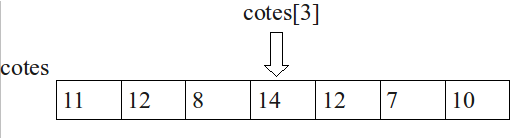
\includegraphics[width=0.8\linewidth,height=0.8\textheight,keepaspectratio=true]{/home/clr/Documents/Cours/DEV1Q2/TDTableau/fr/image/tabPres.png}
						\end{center}
                
                    \caption[tabPres.png]{tabPres.png}
                \end{figure}
                    
            \par
        
        Contrairement \`a algo o\`u on a le choix des valeurs desbornes pour les indices, 
        en Java, les indices varient de \verb@0@ \`a \verb@taille du tableau - 1@.
      
            \par
        0 est l'indice de d\'epart.
            \par
        
			
		\subparagraph{D\'eclaration et cr\'eation : 2 \'etapes} 
		
					\textcolor{white}{.} \par
				
        En Java, l'\'etape de cr\'eation est s\'epar\'ee de l'\'etape de d\'eclaration. \par
				
        En effet, l'\'etape de d\'eclaration r\'eserve un emplacement m\'emoire sur la pile qui contiendra une adresse 
        o\`u trouver la valeur des \'el\'ements du tableau. 
        La cr\'eation connaitra lataille du tableau, le cr\'eera sur le tas et remplira l'adresse sur la pile.
      
            \par
        \begin{figure}[hbt]
				    \begin{center}
					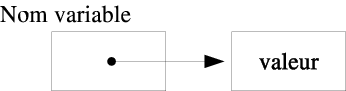
\includegraphics[width=0.8\linewidth,height=0.8\textheight,keepaspectratio=true]{/home/clr/Documents/Cours/DEV1Q2/TDTableau/fr/image/reference.png}
						\end{center}
                
                    \caption[reference.png]{reference.png}
                \end{figure}
                    
            \par
        
			
		\subparagraph{D\'eclaration} 
		
					\textcolor{white}{.} \par
				
        Pour d\'eclarer un tableau : 
      
            \par
        \begin{verbatim}
Type[] identifier
      \end{verbatim}
        Par exemple :\par
				\verb@int []@ est le type tableau d'entiers\par
				\verb@String []@ est le type tableau de chaines de caract\`eres
      
            \par
        \begin{verbatim}
int [] cotes ;
String [] noms;
      \end{verbatim}
			
		\subparagraph{Cr\'eation} 
		
					\textcolor{white}{.} \par
				
        Pour cr\'eer un tableau : 
      
            \par
        \begin{verbatim}
identifier = new Type[taille]
      \end{verbatim}
        Par exemple :\par
				\verb@new int[3]@\par
				\verb@new String[taille]@ o\`u \verb@taille@ est d\'efini
      
            \par
        \begin{verbatim}
int [] entiers ; // déclaration
entiers = new int[3]; // création
      \end{verbatim}
        La d\'eclaration et la cr\'eation peuvent \^etre combin\'ees
      
            \par
        \begin{verbatim}
int [] entiers = new int[3];
      \end{verbatim}
			
		\subparagraph{Initialisation} 
		
					\textcolor{white}{.} \par
				
        Par d\'efaut, les \'el\'ements sont initialis\'es \`a 0 (num\'eriques) ou false (bool\'eens).
        Ce ne sont pas forc\'ement les valeurs initiales que nous d\'esirons. Pour changer \c ca :
      
            \par
        \begin{verbatim}
identifier = new Type[] {x, x}
      \end{verbatim}
        Par exemple :\par
				\verb@new int[] {42, 17, -5}@\par
				\verb@new String[] {"foo", "bar"}@
            \par
        \begin{verbatim}
int [] entiers = new int[] {0x2A, 021, −5};
String [] noms = new String[] {" Victoria ", "Melanie", "Melanie", "Emma", "Geri"};
double[] réels ;
réels = new double[] {4.2, −1};
      \end{verbatim}
			
		\subparagraph{Cas particulier : d\'eclaration, cr\'eation et initialisation} 
		
					\textcolor{white}{.} \par
				
        On peut d\'eclarer le tableau, le cr\'eer et l'initialiser en une seule \'etape, en donnant ses valeurs :
      
            \par
        \begin{verbatim}
int [] entiers = {0x2A, 021, −5};
double[] pseudoRéels = {4.5, 1E−4, −4.12, Math.PI};

// Mais si sur 2 lignes :
double[] réels ;
réels = {4.2, −1}; // FAUX
      \end{verbatim}
			
		\subparagraph{Acc\`es aux \'el\'ements} 
		
					\textcolor{white}{.} \par
				
					\begin{enumerate}
				
			\item 0 est l'indice de d\'epart
			\item les indices varient de 0 \`a taille du tableau - 1
			\item la taille du tableau est son nombre d'\'el\'ements
					\end{enumerate}
				
            \par
        \begin{verbatim}
int [] entiers = {3, 14, 15};
int entier = entiers [2]; // entier vaut 15
entiers [1] = 85;
entier = 0;
entier = entiers [ entier +1]; // entier vaut 85
      \end{verbatim}Par exemple :
            \par
        \begin{verbatim}

package be.heb.esi. lg1 . tutorials . tableaux ;

public class InitialisationTableau {
    public static void main(String [] args) {
      int [] entiers = new int[10];
      for(int i = 0; i < 10; i++) {
        entiers [ i ] = i;
      }
    }
}\end{verbatim}\subsection{Taille logique et physique}
		    Parfois, on connait la taille d'un tableau lorsqu'on \'ecrit l'algorithme (par exemple s'il s'agit
        de retenir les ventes pour les douze mois de l'ann\'ee) mais ce n'est pas toujours le cas (par
        exemple, connait-on le nombre de produits vendus par le magasin ?).
		  
            \par
        
		    Si cette taille n'est pas connue, une possibilit\'e est
        d'attribuer au tableau une taille maximale (sa taille physique) et de retenir dans une
        variable le nombre r\'eel de cases utilis\'ees (sa taille logique).
		  
            \par
        \begin{verbatim}
// Calcule et affiche la quantité vendue de x produits.
module statistiquesVentes()
    cpt : tableau [1 à 1000] d’entiers
    i, numéroProduit, quantité : entiers
    nbArticles : entier
    
    lire nbArticles
    pour i de 1 à nbArticles faire
      cpt[i] ← 0
    fin pour
    
    afficher "Introduisez le numéro du produit :"
    lire numéroProduit
    tant que numéroProduit > 0 ET numéroProduit <= nbArticles faire
      afficher "Introduisez la quantité vendue :"
      lire quantité
      cpt[numéroProduit] ← cpt[numéroProduit] + quantité
      afficher "Introduisez le numéro du produit :"
      lire numéroProduit
    fin tant que
    
    pour i de 1 à nbArticles faire
      afficher "quantité vendue de produit ", i, " : ", cpt[i]
    fin pour
fin module
\end{verbatim}\subsection{Taille d'un tableau en Java}
		    En Java, un tableau connait sa taille
      
            \par
        \begin{verbatim}
identifier.length
      \end{verbatim}\begin{verbatim}
int [] entiers = {4, 5, 6};
int taille = entiers . length ;
System.out. println ( taille ); // écrit 3
      \end{verbatim}Par exemple : 
            \par
        \begin{verbatim}
package be.heb.esi. lg1 . tutorials . tableaux ;

public class SimpleParcoursAscendant {
    public static void main(String [] args){
      int [] entiers = {1, 2, 3, 4, 5, 6, 7, 8, 9, 10};
      for(int i = 0; i < entiers . length ; i = i + 1) {
        System.out. println ( entiers [ i ]);
      }
    }
}
      \end{verbatim}ou encore
            \par
        \begin{verbatim}
package be.heb.esi. lg1 . tutorials . tableaux ;

public class SimpleParcoursDescendant {
    public static void main(String [] args){
      int [] entiers = {1, 2, 3, 4, 5, 6, 7, 8, 9, 10};
      for(int i = entiers . length − 1; i >= 0; i = i−1) {
        System.out. println ( entiers [ i ]);
      }
    }
}
      \end{verbatim}\subsection{Tableau et param\`etres de module}
		    Un tableau peut \^etre pass\'e en param\`etre \`a un module mais qu'en est-il de sa taille ? Il
        serait utile de pouvoir appeler le m\^eme module avec des tableaux de tailles diff\'erentes. Pour
        permettre cela, la taille du tableau re\c cu en param\`etre est d\'eclar\'ee avec une variable (qui
        peut \^etre consid\'er\'e comme un param\`etre entrant).
		  
            \par
        
		    Par exemple :
		  
            \par
        \begin{verbatim}
module afficherTaille(tabEntier↓ : tableau [1 à n] d’entiers)
    afficher "J’ai reçu un tableau de ", n, " éléments".
fin module
      \end{verbatim}
        Ce \verb@n@ va prendre la taille pr\'ecise du tableau utilis\'e \`a chaque appel
        et peut \^etre utilis\'e dans le corps du module. Bien s\^ur il s'agit l\`a de la 
        \textbf{taille physique} du tableau. 
      
            \par
        
        Si une partie seulement du tableau doit \^etre trait\'ee, il convient de \textbf{passer \'egalement
        la taille logique en param\`etre}.
      
            \par
        Par exemple :
            \par
        \begin{verbatim}
module afficherTailles(tabEntiers↓ : tableau [1 à n] d’entiers, tailleLogique : entier)
    afficher "J’ai reçu un tableau rempli de ", tailleLogique, " éléments "
    afficher "sur ", n, " éléments au total."
fin module
      \end{verbatim}
        Un module peut retourner un tableau.
      
            \par
        \begin{verbatim}
// Crée un tableau statique d’entiers de taille 10, l’initialise à 0 et le retourne.
module créerTableau() → tableau [1 à 10] d’entiers
    tab : tableau [1 à 10] d’entiers
    i : entier
    pour i de 1 à 10 faire
      tab[i] ← 0
    fin pour
    retourner tab
fin module

module principalAppelTableau()
    entiers : tableau [1 à 10] d’entiers
    i : entier
    entiers ← créerTableau()
    pour i de 1 à 10 faire
      afficher entiers[i]
    fin pour
fin module
      \end{verbatim}
        Attention, il n'est pas possible de lire ou d'afficher un tableau en une seule instruction ; il faut des
        instructions de lecture ou d'affichage individuelles pour chacun de ses \'el\'ements.
      
            \par
        \subsection{Tableau et param\`etres de m\'ethodes}Un tableau peut \^etre un param\`etre d'une m\'ethode.
            \par
        Par exemple :
            \par
        \begin{verbatim}
public static void afficher ( int [] entiers ) {
    for(int i = 0; i <entiers . length ; i ++) {
      System.out. println ( entiers [ i ]);
    }
}\end{verbatim}L'appel pourrait \^etre
            \par
        \begin{verbatim}
int [] cotes = {12, 8, 10, 14, 9};
afficher ( cotes );
      \end{verbatim}
			
		\subparagraph{Passage de param\`etre par valeur} 
		
					\textcolor{white}{.} \par
				
        En Java, passage de param\`etre par valeur.
        Pour un tableau, cela signifie que l'on ne peut pas
        modifier le tableau dans son ensemble mais que
        l'on pourra modifier ses \'el\'ements.
      
            \par
        Par exemple :
            \par
        \begin{verbatim}
public static void remplir ( int [] entiers , int val ) {
    for(int i = 0; i <entiers . length ; i ++) {
      entiers [ i ] = val;
    }
}\end{verbatim}L'appel pourrait \^etre
            \par
        \begin{verbatim}
int [] cotes = new int[16]; // Ne pas oublier de le créer !
remplir ( cotes , 20 );
      \end{verbatim}MAIS :
            \par
        \begin{verbatim}
public static void méthodeFausse( double[] réels ) {
    double[] réelsDePassage = {4.2, −7, Math.PI};
    réels = réelsDePassage; // INUTILE
}\end{verbatim}
        Quel que soit l'appel, le tableau que l'on passe en
        param\`etre ne sera pas modifi\'e.
      
            \par
        
			
		\subparagraph{Un tableau peut \^etre une valeur de retour} 
		
					\textcolor{white}{.} \par
				
            \par
        Par exemple :
            \par
        \begin{verbatim}
ppublic static int [] créer ( int taille , int val ) {
    int [] entiers = new int[ taille ];
    for(int i = 0; i < taille ; i ++) {
      entiers [ i ] = val;
    }
    return entiers ;
}\end{verbatim}L'appel pourrait \^etre
            \par
        \begin{verbatim}
int [] cotes = créer(16, 20);
      \end{verbatim}\subsection{Parcours d'un tableau \`a une dimension.}
		    Soit le tableau \verb@tab@ d\'eclar\'e ainsi
		  
            \par
        \begin{verbatim}
tab : tableau [1 à n] de T  // où T est un type quelconque
      \end{verbatim}Envisageons d'abord le parcours complet et voyons ensuite les parcours avec arr\^et pr\'ematur\'e.
            \par
        
			
		\subparagraph{Parcours complet.} 
		
					\textcolor{white}{.} \par
				
		    Pour parcourir compl\`etement un tableau, on peut utiliser la boucle 
		    \verb@pour@ comme dans
        l'algorithme suivant o\`u \guillemotleft  traiter \guillemotright  va d\'ependre du probl\`eme concret pos\'e : afficher, modifier,
        sommer, . . .
      
            \par
        \begin{verbatim}
// Parcours complet d’un tableau via une boucle pour
// Les déclarations sont omises pour ne pas alourdir les algorithmes.
pour i de 1 à n faire
    traiter tab[i]
fin pour
      \end{verbatim}
			
		\subparagraph{Parcours avec sortie pr\'ematur\'ee.} 
		
					\textcolor{white}{.} \par
				
        Parfois, on ne doit pas forc\'ement parcourir le tableau jusqu'au bout mais on pourra s'arr\^eter
        pr\'ematur\'ement si une certaine condition est remplie. Par exemple :
        
					\begin{enumerate}
				
			\item on cherche la pr\'esence d'un \'el\'ement et on vient de le trouver ;
			\item on v\'erifie qu'il n'y a pas de 0 et on vient d'en trouver un.
					\end{enumerate}
				
        La premi\`ere \'etape est de transformer le \verb@pour@ 
        en \verb@tant que@ ce qui donne l'algorithme
      
            \par
        \begin{verbatim}
// Parcours complet d’un tableau via une boucle tant-que
i ← 1
tant que i ≤ n faire
    traiter tab[i]
    i ← i+1
fin tant que
		  \end{verbatim}
		    On peut \`a pr\'esent introduire le test d'arr\^et. Une contrainte est qu'on voudra, \`a la fin de la
        boucle, savoir si oui ou non on s'est arr\^et\'e pr\'ematur\'ement et, si c'est le cas, \`a quel indice.
      
            \par
        
        Il existe essentiellement deux solutions, avec ou sans variable bool\'eenne. En g\'en\'eral, la
        solution [A] sera plus claire si le test est court.
		  
            \par
        
			
		\subparagraph{Parcours avec sortie pr\'ematur\'ee sans variable bool\'eenne} 
		
					\textcolor{white}{.} \par
				
            \par
        \begin{verbatim}
// Parcours partiel d’un tableau sans variable booléenne
i ← 1
tant que i ≤ n ET test sur tab[i] dit que on continue faire
    i ← i+1
fin tant que

si i > n alors
    // on est arrivé au bout
sinon
    // arrêt prématuré à l’indice i.
fin si
      \end{verbatim}
        Il faut \^etre attentif \`a \textbf{ne pas inverser les deux parties du test}. 
        Il faut absolument v\'erifier  que l'indice est bon avant de tester la valeur \`a cet indice.
      
            \par
        
        On pourrait inverser les deux branches du si-sinon en inversant le test mais attention \`a ne
        pas tester \verb@tab[i]@ car \verb@i@ n'est peut-\^etre pas valide.
      
            \par
        
        Dans certains cas, le si-sinon peut se simplifier en un simple return d'une condition.
      
            \par
        Par exemple : 
            \par
        \begin{verbatim}
// Indique si un zéro est présent dans le tableau
module contientZéro(tab : tableau [1 à n] d’entiers) → booléen
    i : entier
    i ← 1
    tant que i ≤ n ET tab[i] ≠ 0 faire
      i ← i+1
    fin tant que
    retourner i ≤ n // Si le test est vrai c’est qu’on a trouvé un 0
fin module
      \end{verbatim}
			
		\subparagraph{Parcours avec sortie pr\'ematur\'ee avec variable bool\'eenne} 
		
					\textcolor{white}{.} \par
				
            \par
        \begin{verbatim}
// Parcours partiel d’un tableau avec variable booléenne
i ← 1
trouvé ← faux
tant que i ≤ n ET NON trouvé faire
    si test sur tab[i] dit que on a trouvé alors
      trouvé ← vrai
    sinon
      i ← i+1
    fin si
fin tant que
// tester le booléen pour savoir si arrêt prématuré.
      \end{verbatim}
        Attention \`a bien choisir un nom de bool\'een adapt\'e au probl\`eme et \`a l'initialiser \`a la bonne
        valeur. Par exemple, si la variable s'appelle \guillemotleft  continue \guillemotright 
        
					\begin{enumerate}
				
			\item initialiser la variable \`a vrai ;
			\item le test de la boucle est \guillemotleft  . . .ET continue \guillemotright  ;
			\item mettre la variable \`a faux pour sortir de la boucle.
					\end{enumerate}
				
            \par
        \subsection{Erreurs fr\'equentes et exceptions lanc\'ees en Java}
					\begin{enumerate}
				
			\item \verb@NullPointerException@ : 
            si vous essayez d'acc\'eder \`a un \'el\'ement d'un tableau qui n'a pas \'et\'e cr\'e\'e
            (le tableau vaut null dans ce cas) ;
          
			\item \verb@ArrayIndexOutOfBoundsException@ : 
            si vous donnez un indice qui n'existe pas (ex : tab [10] quand il n'y a que 10 \'el\'ements dans le tableau).
          
					\end{enumerate}
				
            \par
        \section{Les tests}\subsection{Tests unitaires}
			
		\subparagraph{Les tests unitaires} 
		
					\textcolor{white}{.} \par
				
          Tous les programmes r\'eels contiennent des bugs (erreurs, d\'efauts), parfois m\^eme beaucoup.
          C'est inacceptable :
          
					\begin{itemize}
				
			\item Inconfort pour l'utilisateur
			\item Perte de temps, d'argent, de donn\'ees, de mat\'eriel
			\item Voire danger pour la vie humaine, par exemple : l'\'echec du vol d'Ariane 5 (\url{fr.wikipedia.org/wiki/Vol\_501\_d\%27Ariane\_5}).
					\end{itemize}
				
            \par
        
          On peut trouver diff\'erents types d'erreurs : 
          
					\begin{itemize}
				
			\item \`a la compilation
			\item \`a l'ex\'ecution, le programme s'arr\^ete
			\item \`a l'ex\'ecution, le programme fournit une mauvaise r\'eponse
					\end{itemize}
				
          On pourrait aussi parler d'autres d\'efauts
          
					\begin{itemize}
				
			\item Trop lent
			\item Trop gourmand en m\'emoire
					\end{itemize}
				
            \par
        
        Pour produire un logiciel sans bug il faut
         
					\begin{itemize}
				
			\item 
              suivre une m\'ethodologie \'eprouv\'ee pour produire une premi\`ere version avec peu de bugs
              (cf. Analyse)
            
			\item 
              tester, tester et . . . tester encore ! Pour d\'etecter ceux qui restent
              
					\begin{itemize}
				
			\item Besoin d'outils pour nous aider de fa\c con \`a tester de la mani\`ere la plus facile/rapide possible
			\item Il existe plusieurs sortes de tests : unitaires, d'int\'egration, fonctionnels, non-r\'egression, . . .
			\item Nous nous int\'eressons aux tests unitaires (\url{fr.wikipedia.org/wiki/Test\_(informatique)}) : 
                c'est une proc\'edure permettant de tester le bon fonctionnement d'un module (une m\'ethode), ce qui n'est pas forc\'ement suffisant.
					\end{itemize}
				
					\end{itemize}
				
            \par
        
			
		\subparagraph{Le plan de tests} 
		
					\textcolor{white}{.} \par
				
          Il faut planifier les tests, c'est-\`a-dire se demander quoi tester en choisissant les cas int\'eressants / judicieux.
          Pour \c ca, il faut se baser sur les erreurs fr\'equentes et cela viendra avec l'exp\'erience.
        
            \par
        
          Nous avons besoin d'un plan reprenant les tests \`a effectuer
          
					\begin{itemize}
				
			\item Quelles valeurs de param\`etres sont pertinentes ?
			\item Quel est le r\'esultat attendu ?
					\end{itemize}
				
          Ce plan de tests doit \^etre pr\'epar\'e pendant que l'on code 
          (ou m\^eme avant et \'eventuellement par une autre personne).
        
            \par
        
          Il permet de s'assurer que l'on teste tous les cas pertinents.
        
            \par
        
          On ne peut pas tester toutes les valeurs possibles
          
					\begin{itemize}
				
			\item Il faut choisir des valeurs repr\'esentatives
              
					\begin{itemize}
				
			\item Cas g\'en\'eral / particuliers
			\item Valeurs limites
					\end{itemize}
				
			\item Il faut imaginer les cas qui pourraient mettre en \'evidence un d\'efaut de la m\'ethode : 
            on s'inspire des erreurs les plus fr\'equentes en programmation :
            
					\begin{itemize}
				
			\item On commence/arr\^ete trop t\^ot/tard une boucle
			\item On initialise mal une variable
			\item Dans un test, on se trompe entre < et ≤
			\item Dans un test, on se trompe entre ET et OU
			\item ...
					\end{itemize}
				
            C'est un savoir-faire ⇒ Importance de l'exp\'erience
            
					\end{itemize}
				
            \par
        
          Par exemple : \verb@public static int max(int n1, int n2, int n3) ...@
          qui calcule la valeur maximale de trois nombres.
        
            \par
        
          Que tester en plus du cas g\'en\'eral ?
          
					\begin{itemize}
				
			\item Le maximum est la premi\`ere/derni\`ere valeur
			\item Pr\'esence de nombres n\'egatifs
					\end{itemize}
				
            \par
        
          Par exemple : plan de tests de la m\'ethode \verb@max@ : 
        
            \par
        \begin{verbatim}
#   nombres     résultat     ce qui est testé
1   1, 3, 0          3        cas général
2   1, −3, −4        1        maximum au début
3   1, 3, 11        11        maximum à la fin
4   −1, −3, −4      −1        que des négatifs
        \end{verbatim}
					\begin{itemize}
				
			\item Quand tester ? 
              
					\begin{itemize}
				
			\item Le plus souvent possible
			\item Erreur plus facile \`a identifier/corriger
			\item Id\'ealement apr\`es chaque m\'ethode \'ecrite
					\end{itemize}
				
			\item Que tester ? 
              
					\begin{itemize}
				
			\item Tout
			\item Le nouveau code peut mettre en \'evidence un probl\`eme dans le code ancien (r\'egression)
					\end{itemize}
				
			\item Comment tester ? 
              
					\begin{itemize}
				
			\item Pas \`a la main : intenable
			\item Besoin d'un outil automatis\'e : \textbf{JUnit}
					\end{itemize}
				
					\end{itemize}
				
            \par
        
			
		\subparagraph{JUnit} 
		
					\textcolor{white}{.} \par
				
          JUnit : outil pour automatiser les tests unitaires :
          
					\begin{itemize}
				
			\item Le programmeur fournit les tests,
			\item JUnit ex\'ecute tous les tests et
			\item \'etablit un rapport d\'etaillant les probl\`emes
					\end{itemize}
				
            \par
        
          La classe de test contient une m\'ethode de test par cas. Cette m\'ethode
          
					\begin{itemize}
				
			\item est autonome (ne re\c coit rien ne retourne rien)
			\item contient des affirmations
			\item fait appel \`a la m\'ethode \`a tester
			\item compare le r\'esultat attendu et le r\'esultat obtenu
					\end{itemize}
				
            \par
        \begin{figure}[hbt]
				    \begin{center}
					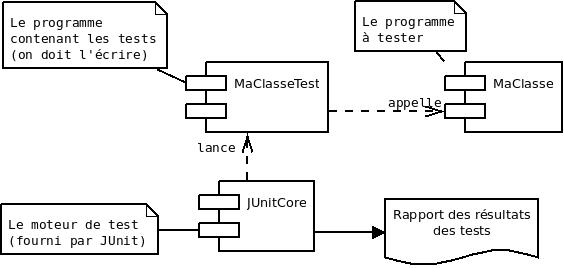
\includegraphics[width=0.8\linewidth,height=0.8\textheight,keepaspectratio=true]{/home/clr/Documents/Cours/DEV1Q2/TDTableau/fr/image/junit.jpeg}
						\end{center}
                
                    \caption[junit.jpeg]{junit.jpeg}
                \end{figure}
                    
            \par
        Par exemple
            \par
        \begin{verbatim}
@Test
public void max_cas1() {
    int n1 = 1, n2 = 3, n3 = 0;
    assertEquals ( 3, MaClasse.max(n1, n2, n3) );
}
\end{verbatim}
					\begin{itemize}
				
			\item Reconnu comme un test unitaire gr\^ace \`a l'annotation \verb@@Test@
			\item Pas de \verb@static@
			\item \verb@assertEquals@ v\'erifie que les 2 valeurs sont identiques
			\item \verb@assertTrue ( val )@, \verb@assertFalse ( val )@, . . .
					\end{itemize}
				
            \par
        
			
		\subparagraph{Lancer les tests} 
		
					\textcolor{white}{.} \par
				
            \par
        
					Pour lancer le test, il suffit de compiler la classe de test puis de lancer la commande : 
					\verb@java org.junit.runner.JUnitCore package.MaClasseTest@.
				
            \par
        
					Cette commande lance les tests 
					et affiche un message r\'ecapitulatif du nombre de tests
					et du d\'ecompte de ceux qui ont r\'eussi ou \'echou\'e.
				
            \par
        
					Si cela ne fonctionne pas directement sur linux1 
					c'est que la JVM ne trouve pas la classe
					\verb@org.junit.runner.JUnitCore@ 
					qui se trouve dans le fichier 
					\textit{jar}\verb@/usr/share/java/junit4.jar@.
					Il faudra donc ajouter ce chemin 
					\`a votre \verb@CLASSPATH@ 
					et relancer un \textit{shell} 
					afin que la variable d'environnement soit relue.
				
            \par
        
					Certains d'entre vous ne voudront pas 
					entrer cette longue commande lors de chaque 
					lancement de tests.    
					Rien ne les emp\^eche de d\'efinir un 
					\textit{alias} avec la commande :
				
            \par
        \begin{verbatim}
	alias javatest='java org.junit.runner.JUnitCore'
				\end{verbatim}
					et ils n'auront plus alors qu'\`a ex\'ecuter la commande
					\verb@javatest package.MaClasseTest@
					pour lancer la classe de tests.
				
            \par
        \section{Exercices}
				Maintenant, mettons tout \c ca en pratique.
      
            \par
        \subsection{En Java...}
			
		\subparagraph{Bornes d'un tableau} 
		
                \textcolor{white}{.} \par
            
					\begin{itemize}
				
			\item 
									La variable permettant de se d\'eplacer dans un tableau s'appelle un  \textcolor{gray}{\underline{\hspace*{5em}}} 
			\item 
									En Java, la premi\`ere valeur d'un tableau \`a \textbf{n} \'el\'ements se trouve \`a la position            
									 \textcolor{gray}{\underline{\hspace*{1em}}}  
									et la derni\`ere valeur se trouve \`a la position 
									 \textcolor{gray}{\underline{\hspace*{2em}}} 
					\end{itemize}
				
			
		\subparagraph{D\'eclaration, cr\'eation et initialisation d'un tableau } 
		
					\textcolor{white}{.} \par
				
            \par
        
					Un tableau poss\`ede un type et une taille.
					Le type de ses \'el\'ements est soit l'un des types simples (int, double, char,..) ou une r\'eference (String,...).
				
            \par
        
					La taille du tableau est le nombre (strictement positif ) de ses \'el\'ements.
					Elle ne fait pas partie du type.  
				
            \par
        La d\'eclaration d'un tableau r\'eserve un emplacement m\'emoire
            \begin{itemize} 
        
            \item[ \ding{"6D} ] sur le tas.
        
            \item[ \ding{"6D} ] sur la pile.
        
            \end{itemize} 
        
			
		\subparagraph{Cr\'eation} 
		
                \textcolor{white}{.} \par
            
								Pour cr\'eer un tableau, le mot cl\'e utilis\'e est  \textcolor{gray}{\underline{\hspace*{2em}}} 
            \par
        
								Pour pouvoir cr\'eer un tableau nomm\'e \textbf{entiers} 
								de 10 entiers \textbf{pr\'ec\'edemment d\'eclar\'e}, il faut \'ecrire l'instruction
								 \textcolor{gray}{\underline{\hspace*{5em}}}  \textcolor{gray}{\underline{\hspace*{1em}}}  \textcolor{gray}{\underline{\hspace*{2em}}}  \textcolor{gray}{\underline{\hspace*{2em}}}  \textcolor{gray}{\underline{\hspace*{3em}}} ;
							
            \par
        La cr\'eation d'un tableau se fait
            \begin{itemize} 
        
            \item[ \ding{"6D} ] sur le tas
        
            \item[ \ding{"6D} ] sur la pile
        
            \end{itemize} 
        
			
		\subparagraph{Initialisation} 
		
                \textcolor{white}{.} \par
            
								Le mot cl\'e \verb|new| permet \'egalement d'initialiser
								tous les \'el\'ements du tableau fraichement cr\'e\'e \`a une valeur par d\'efaut. 
							
            \par
        Quelle est cette valeur par d\'efaut ?
            \par
        
					\begin{itemize}
				
			\item pour les num\'eriques (int, double, char) :  \textcolor{gray}{\underline{\hspace*{1em}}} 
			\item pour les boolean :  \textcolor{gray}{\underline{\hspace*{3em}}} 
			\item pour les objets (type r\'eference) :  \textcolor{gray}{\underline{\hspace*{3em}}} 
					\end{itemize}
				
			
		\subparagraph{R\'eflexion} 
		
					\textcolor{white}{.} \par
				
            \par
          
					Est-il possible de d\'eclarer, de cr\'eer et d'initialiser un tableau de 10 \'el\'ements en une seule op\'eration ?  
				
            \par
         {\footnotesize\emph{(la r\'eponse est disponible dans la version en ligne)}\par} 
			
		\subparagraph{V\'erification} 
		
					\textcolor{white}{.} \par
				
            \par
        
					\'Ecrivez sur papier la boucle permettant d'initialiser
					les \'el\'ements d'un tableau d'entiers de 10 \'el\'ements \`a la valeur de leur indice.   
				
            \par
         {\footnotesize\emph{(la r\'eponse est disponible dans la version en ligne)}\par} 
			
		\subparagraph{Cochez les affirmations qui sont vraies} 
		
                \textcolor{white}{.} \par
            
							Considerons le tableau \verb|entiers|
							contenant les \'elements \verb|{3,4,5}|.
						
            \begin{itemize} 
        
            \item[ \ding{"6F} ] 
							Le tableau connait sa taille.
						
        
            \item[ \ding{"6F} ] \verb|entiers[3]| vaut 5.
						
        
            \item[ \ding{"6F} ] \verb|entiers[3]=4;| affecte la valeur 4 \`a la 3\textsuperscript{\`eme} case.
						
        
            \item[ \ding{"6F} ] \verb|entiers[1]=0;| supprime la case d'indice 1.
						
        
            \item[ \ding{"6F} ] 
							Si \verb|entiers20| est un tableau de 20 entiers, on peut \'ecrire l'instruction 
							\verb|entiers20 = entiers;|.  
						
        
            \item[ \ding{"6F} ] 
							Un tableau peut \^etre le seul param\`etre d'une m\'ethode.
						
        
            \item[ \ding{"6F} ] 
							Un tableau peut \^etre une valeur de retour d'une m\'ethode.
						
        
            \end{itemize} 
        
			
		\subparagraph{S\'election multiple} 
		
                \textcolor{white}{.} \par
            
								Partons de la repr\'esentation de \verb|entiers |en m\'emoire
								donn\'ee par la figure ci-dessous.  
							\begin{figure}[hbt]
				    \begin{center}
					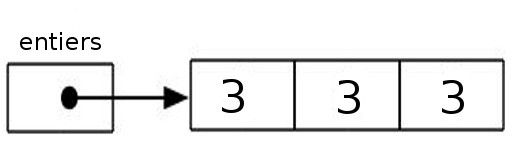
\includegraphics[width=0.5\linewidth,height=0.8\textheight,keepaspectratio=true]{/home/clr/Documents/Cours/DEV1Q2/TDTableau/fr/image/tab3.jpg}
						\end{center}
                
                    \caption[repr\'esentation m\'emoire de entiers]{repr\'esentation m\'emoire de entiers}
                \end{figure}
                    
            \par
        
								Quelle(s) instruction(s) m\`ene(nt) \`a ce r\'esultat.   
							
            \par
        
            \begin{itemize} 
        
            \item[ \ding{"6F} ] proposition 1
            \par
        \begin{Java}
int [] entiers;
entiers = new int [3];
							\end{Java}
        
            \item[ \ding{"6F} ] proposition 2
            \par
        \begin{Java}
int [] entiers = new int [3]; 
							\end{Java}
        
            \item[ \ding{"6F} ] proposition 3
            \par
        \begin{Java}
int [] entiers = new int [];
							\end{Java}
        
            \item[ \ding{"6F} ] proposition 4
            \par
        \begin{Java}
int [] entiers = {3,3,3};
							\end{Java}
        
            \item[ \ding{"6F} ] proposition 5
            \par
        \begin{Java}
int [] entiers = new int [3];
for (int i=0; i<entiers.length; i++) {
	entiers[i] = 3;
}
							\end{Java}
        
            \item[ \ding{"6F} ] proposition 6
            \par
        \begin{Java}
int[] entiers;
entiers = {3,3,3};
							\end{Java}
        
            \item[ \ding{"6F} ] proposition 7
            \par
        \begin{Java}
int [3] entiers = {3,3,3};
							\end{Java}
        
            \item[ \ding{"6F} ] proposition 8
            \par
        \begin{Java}
int [] entiers;
entiers= new {3,3,3};
							\end{Java}
        
            \end{itemize} 
        
			
		\subparagraph{Quiz} 
		
                \textcolor{white}{.} \par
            Pour ce tableau de 3 \'el\'ements, l'instruction \verb|System.out.println (entiers[6]);|
            \begin{itemize} 
        
            \item[ \ding{"6D} ] n'affiche rien.
        
            \item[ \ding{"6D} ] affiche une valeur se trouvant en m\'emoire.
        
            \item[ \ding{"6D} ] provoque une erreur \`a la compilation.
        
            \item[ \ding{"6D} ] provoque une  erreur \`a l'ex\'ecution.
        
            \end{itemize} 
        \subsection{Les tests unitaires}
			
		\subparagraph{Les tests} 
		
                \textcolor{white}{.} \par
                
								Le type de tests qui  teste s\'epar\'ement chaque m\'ethode est appel\'e tests  \textcolor{gray}{\underline{\hspace*{10em}}} .
							
            \par
            
								Avant de commencer \`a tester, il faut \'ecrire un  \textcolor{gray}{\underline{\hspace*{3em}}}  de tests afin de s'assurer qu'on teste tous les cas.
							
            \par
            
								Bien s\^ur, il n'est pas pensable de tester toutes les valeurs possibles, il faut donc choisir des valeurs repr\'esentatives 
								(c-\`a-d cas g\'en\'eral, cas particuliers et valeurs limites).    
							
            \par
         \textcolor{gray}{\underline{\hspace*{3em}}}  est un outil pour automatiser les tests unitaires.
							
            \par
            
								Cette m\'ethode est autonome (ne re\c coit rien ne retourne rien) 
								et elle ne contient que des affirmations 
								(appel de la m\'ethode \`a tester, comparaison entre le r\'esultat attendu et le r\'esultat obtenu).
							
            \par
            
								Une classe de test contient une m\'ethode de test par cas.
								Chaque m\'ethode de test est reconnue comme \'etant un test unitaire gr\^ace au tag  \textcolor{gray}{\underline{\hspace*{3em}}}  .
								Elle contient des affirmations :
							
            \par
        
					\begin{itemize}
				
			\item  \textcolor{gray}{\underline{\hspace*{10em}}} (intAttendu, intObtenu) 
								  v\'erifie que les 2 valeurs enti\`eres \verb|intAttendu| et \verb|intObtenus| sont identiques;
								
            \par
        
			\item  \textcolor{gray}{\underline{\hspace*{10em}}} (val) 
								  v\'erifie que la valeur du bool\'een \verb|val| est \`a vrai,     
                
            \par
        
			\item  \textcolor{gray}{\underline{\hspace*{10em}}} (val) 
								  v\'erifie que la valeur de \verb|val| est \`a faux.    
                
            \par
        
					\end{itemize}
				    
								Le tag  \textcolor{gray}{\underline{\hspace*{3em}}}  ( \textcolor{gray}{\underline{\hspace*{20em}}} )  
                permet de v\'erifier que la m\'ethode lance bien une exception de type \verb|IllegalArgumentException|.    
							
            \par
        
                Dans la classe de tests, 2 instructions \verb|import| sont n\'ecessaires :    
							
					\begin{itemize}
				
			\item import  \textcolor{gray}{\underline{\hspace*{2em}}} . \textcolor{gray}{\underline{\hspace*{3em}}} . \textcolor{gray}{\underline{\hspace*{3em}}} ; 
                // Pour que @Test soit connu
                
			\item import  \textcolor{gray}{\underline{\hspace*{5em}}}  \textcolor{gray}{\underline{\hspace*{2em}}} . \textcolor{gray}{\underline{\hspace*{3em}}} . \textcolor{gray}{\underline{\hspace*{5em}}} . \textcolor{gray}{\underline{\hspace*{1em}}} ; 
                // Pour que les m\'ethodes de v\'erification ci-dessus soient reconnues.
                
					\end{itemize}
				
            \par
            
								La commande
								\par
				 \textcolor{gray}{\underline{\hspace*{3em}}}  \textcolor{gray}{\underline{\hspace*{16em}}}  \textcolor{gray}{\underline{\hspace*{20em}}}  \par
				
								permet de lancer les tests de la classe \verb|ExerciceTest|, 
								dont le package est \verb|g32000.tds.td7BisPrepa|, pr\'ec\'edemment compil\'ee.    
							
            \par
        \subsection{\`A vous de jouer...}
          N'oubliez pas nos quelques conseils pour vous guider dans la r\'esolution de tels probl\`emes :
          
					\begin{itemize}
				
			\item il convient d'abord de bien comprendre le probl\`eme pos\'e ; assurez-vous qu'il est parfaitement sp\'ecifi\'e ;
			\item r\'esolvez le probl\`eme via quelques exemples pr\'ecis ;
			\item mettez en \'evidence les variables \textbf{\guillemotleft  donn\'ees \guillemotright }, les variables \textbf{\guillemotleft  r\'esultats \guillemotright } et les variables de travail ;
			\item n'h\'esitez pas \`a faire une \'ebauche de r\'esolution en fran\c cais avant d'\'elaborer l'algorithme d\'efinitif pseudo-cod\'e ;
			\item d\'eclarez ensuite les variables (et leur type) qui interviennent dans chaque module ; les noms des variables risquant de ne pas \^etre suffisamment explicites.
			\item \'Ecrivez la partie algorithmique \textbf{AVANT} de vous lancer dans la programmation en Java.
			\item Demandez-vous si vous avez besoin de parcourir tout le tableau ou de sortir pr\'ematur\'ement (si on a trouv\'e ce qu'on cherche par exemple).
			\item Pour la partie Java, dessinez l'arborescence des fichier. 
			\item \textbf{\'Ecrivez le plan de tests en \'ecrivant l'algorithme. Codez les tests apr\`es avoir \'ecrit le code Java.}
					\end{itemize}
				
            \par
        
        \'Ecrivez les algorithmes et codez les programmes Java correspondant qui 
          
					\begin{enumerate}
				
			\item  re\c coit en param\`etre le tableau \verb@températures@ de 
              \verb@n@  r\'eels et qui retourne
              le plus grand \'ecart absolu entre deux temp\'eratures cons\'ecutives de ce tableau. Et si on veut
              le plus petit \'ecart ?
            
			\item 
              re\c coit en param\`etre le tableau valeurs de \verb@n@ entiers et qui v\'erifie si ce
              tableau est ordonn\'e (strictement) croissant sur les valeurs. Le module retournera vrai si le
              tableau est ordonn\'e, faux sinon.
            
			\item 
              re\c coit en param\`etre le tableau \verb@tabCar@ 
              de \verb@n@ caract\`eres, et qui \guillemotleft  renverse \guillemotright 
              ce tableau, c'est-\`a-dire qui permute le premier \'el\'ement avec le dernier, le deuxi\`eme \'el\'ement
              avec l'avant-dernier et ainsi de suite.
              
			\item 
              re\c coit en param\`etre le tableau \verb@tabChaines@ 
              de \verb@n@ chaines et qui v\'erifie
              si ce tableau est sym\'etrique, c'est-\`a-dire si le premier \'el\'ement est identique au dernier, le
              deuxi\`eme \`a l'avant-dernier et ainsi de suite.
            
			\item 
              re\c coit un nombre entier positif ou nul en param\`etre et qui affiche pour
              chacun de ses chiffres le nombre de fois qu'il apparait dans ce nombre. Ainsi, pour le nombre
              10502851125, l'affichage mentionnera que le chiffre 0 apparait 2 fois, 1 apparait 3 fois, 2
              apparait 2 fois, 5 apparait 3 fois et 8 apparait une fois (l'affichage ne mentionnera donc pas
              les chiffres qui n'apparaissent pas).
            
			\item 
              v\'erifie si un tableau d' entiers donn\'e forme un palindrome ou non. Un nombre
              palindrome est un nombre qui lu dans un sens (de gauche \`a droite) est identique au nombre
              lu dans l'autre sens (de droite \`a gauche). Par exemple, 1047401 est un nombre palindrome.
            
					\end{enumerate}
				
            \par
        En java, n'oubliez pas d'\'ecrire la javadoc et les tests de vos m\'ethodes.
            \par
        
			
		\subparagraph{Mastermind} 
		
					\textcolor{white}{.} \par
				
          Dans le jeu du Mastermind, un joueur A doit trouver une combinaison de 
          \verb@k@ pions de couleur,
          choisie et tenue secr\`ete par un autre joueur B. Cette combinaison peut contenir \'eventuellement 
          des pions de m\^eme couleur. \`A chaque proposition du joueur A, le joueur B indique
          le nombre de pions de la proposition qui sont corrects et bien plac\'es et le nombre de pions
          corrects mais mal plac\'es.
        
            \par
        
          Pour impl\'ementer une simulation de ce jeu, on utilise le type Chaine, dont les valeurs
          possibles sont les couleurs des pions utilis\'es. (Attention, le nombre exact de couleurs n'est
          pas pr\'ecis\'e.) Les seules manipulations permises ont la comparaison (tester si
          deux couleurs sont identiques ou non) et l'affectation (affecter le contenu d'une variable de
          type Couleur \`a une autre variable de ce type). Les propositions du joueur A, ainsi que la
          combinaison secr\`ete du joueur B sont contenues dans des tableaux de k composantes de type
          Chaine.
        
            \par
        
          \'Ecrire le module suivant qui renvoie dans les variables \verb@bienPlacés@ 
          et \verb@malPlacés@ respectivement
          le nombre de pions bien plac\'es et mal plac\'es dans la \guillemotleft  proposition \guillemotright  du joueur A en la
          comparant \`a la \guillemotleft  solution \guillemotright  cach\'ee du joueur B.
        
            \par
        \begin{verbatim}
module testerProposition( proposition↓, solution↓ : tableau [1 à k ] de Chaines, bienPlacés↑, malPlacés↑ : entiers)
        \end{verbatim} {\footnotesize\emph{(une solution est disponible dans la version en ligne)}\par} En java, n'oubliez pas d'\'ecrire la javadoc et les tests de vos m\'ethodes.
            \par
        
				\end{document}
			